%!TEX root = /Users/andy/Documents/Academics/Dissertation/thesis.tex
%

\begin{savequote}[75mm] 
This is some random quote to start off the chapter.
\qauthor{Firstname lastname} 
\end{savequote}

\chapter{Maximum Likelihood Estimator Bayesian Inference DNA Origami  Nanorod Barcode Detection} \label{chapter:DNAtheory}

\section{Introduction}
\newthought{The development of next generation microarray and on-chip technologies} will depend in part upon advancements in fluorescent reporter molecules and improvements in their detection.

Currently accepted microarray techniques  use at most two spectrally distinct fluorophores to identify their targets.  Recently, however, there has been an explosion in fluorescent reporter approaches that enables an observer to uniquely identify one out of many hundreds of distinct fluorescent encoded reporters. Researchers have explored both combining spectrally distinct fluorophores in close proximity to create gradations of colors[cite a bunch of stuff], and spatially separating fluorophores to create geometric optical barcodes [cite a bunch of stuff]. In particular, fluorescently encoded DNA based nanorods [cite the DNA related ones] provide a promising avenue to DNA based micro-array techniques. Instead of identifying DNA microarray targets largely by location, this raises the distinct possibility of also unambiguously identifying targets by fluorescent encoding. 

Programmatically identifying images of these fluorescently encoded barcodes, however, presents unique computational challenges that have not yet been explored in the literature.  Here we describe a mathematical formalism that allows us to use computer vision to optimally detect DNA origami-based nanorod barcodes. We take a bayesian inference approach, and demonstrate that our implementation allows for >blah \% correct barcode identification under real-world situations. 

\section{System and Methods}

\subsection{DNA origami nanorod barcodes}
We chose to image DNA origami nanorod barcodes (see Chapter \ref{chapter:DNAbarcode}). These nanorods consist of mechanically rigid six-helix bundles of DNA with radius 5 nm and length 720 nm decorated with  12 molecules of up to two spectrally distinct fluorophores at each of three distinct locations along the rod, as illustrated in Figure~\ref{fig:cartoonBarcode}. The three fluorescing sites are unevenly spaced, with a large gap of \textasciitilde 450 nm and a small gap of \textasciitilde 270 nm  between the fluorescing sites on each rod, giving the barcodes a visible anisotropy. When using combinations of red, green and blue fluorophores, (Cy5, Cy3 and Alexa Fluor 488, respectively) this allows for a dictionary of six fluorescing symbols at each of the three barcode locations: \{Red, Green, Blue, RedGreen, RedBlue, GreenBlue\}, for a total of $6^{3}=216$  unambiguous species of barcode.

\begin{figure}[htbp]
\begin{center}
	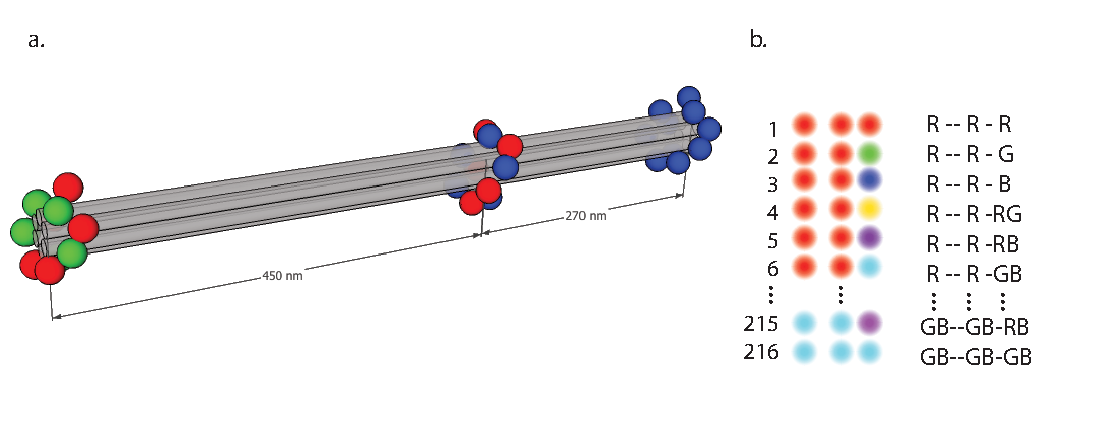
\includegraphics[width=\textwidth]{figures/theoryCartoonBarcode}
	\caption{Cartoon of of DNA origami nanorod barcodes (not to scale) . \textbf{(a)} The barcode is a composed of a six  helix-bundle of DNA, 5 nm in diameter and 720nm long, decorated at three fluorescing sites with 12 molecules of up to two  spectrally distinct fluorophores per site. The barcode has an inherent anisotropy due to the uneven spacing of three fluorescing sites (large gap on the left, smaller gap on the right). The barcode shown is of species RedGreen--RedBlue-Blue. \textbf{(b)} The barcodes use a combination of red (R), green (G), and blue (B) fluorescent molecules, providing a dictionary of six fluorescing symbols at each of the three barcode locations \{R, G, B, RG, RB, GB\}, for a total of $6^{3}=216$ distinct barcode species. In composite images RG appears yellow, RB appears purple and GB appears turquoise.   \label{fig:cartoonBarcode}}
\end{center}	
\end{figure}

We chose to work with this particular form of fluorescently encoded barcodes as opposed to others because this form offer the largest published number of distinct barcode species to date, has the advantage of being massively self-assembled in parallel, and creates barcodes of suitably small  size so as to be useful for future microarray applications. 

The barcodes are, in fact, so small that the distance between fluorescing sites is often smaller than a wavelength of light. As a result, when the barcodes are imaged on a flat surface, the distinct flourescent sites appear to blend into one another (see Figure~\ref{fig:rawImage}). This becomes one of the primary challenges facing any computer vision barcode identification software, namely to  decode the barcode even when there is overlap between individual difraction-limited fluorescent spots. 
\begin{figure}[htbp]
\begin{center}
	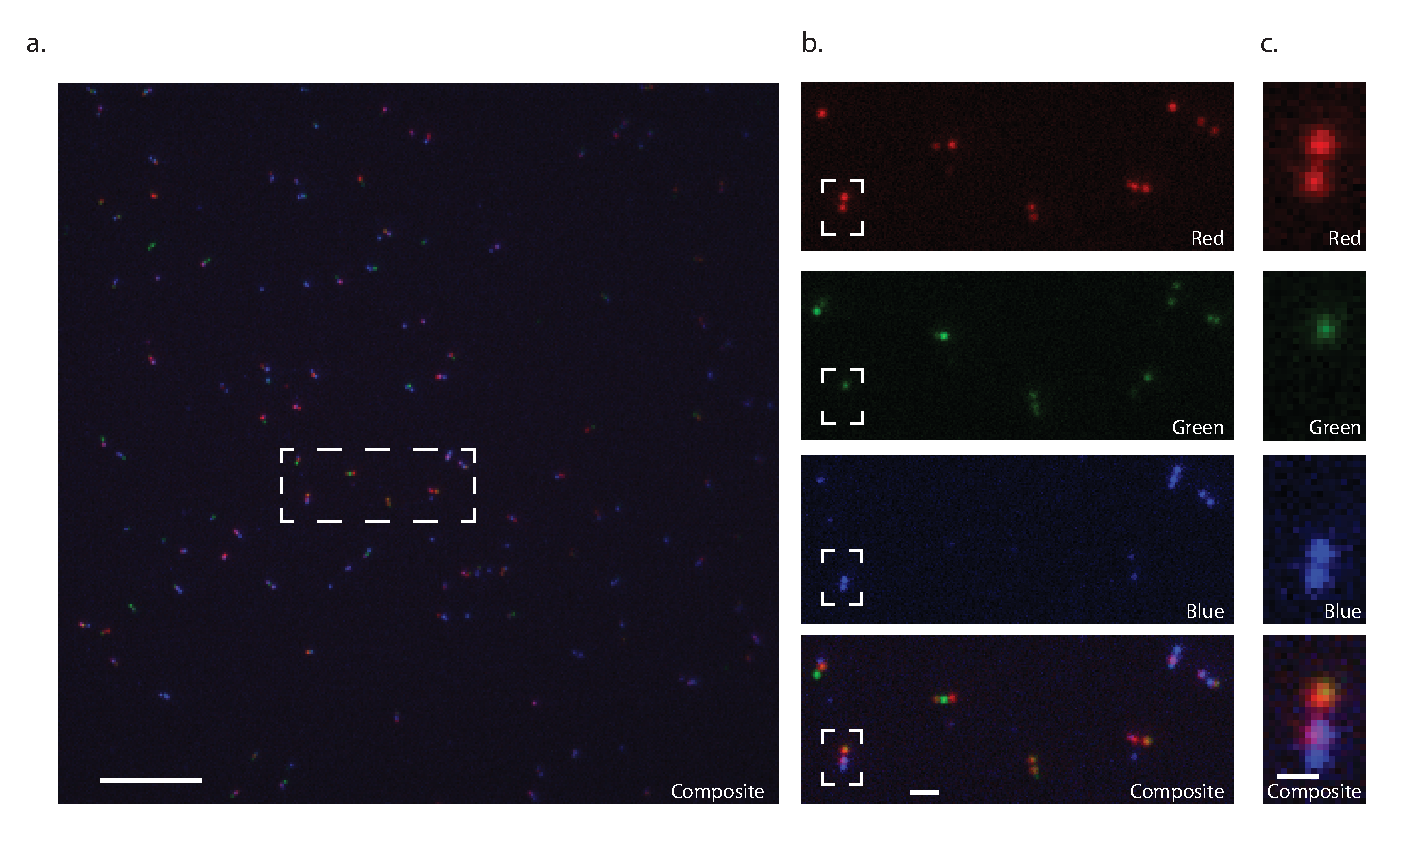
\includegraphics[width=\textwidth]{figures/theoryRawImage}
	\caption{Fluorescent images of DNA origami nanorod barcodes. \textbf{(a)} Composite image. Scale bar is 100 \textmu m. \textbf{(b)} Inset of dashed region in \textbf{a}. Scale bar is 10 \textmu m. \textbf{(c)} A single barcode of species RedGreen--RedBlue-Blue. (Inset of dashed region in \textbf{c}.) Scale bar is 500 nm. \label{fig:rawImage}}
\end{center}	
\end{figure}


\subsection{Imaging}
Barcodes were imaged on a glass cover slide on a Leica DM1600 microscope using a 100x oil-immersion objective,  under total internal reflection fluorescence (TIRF) . 
The red, green and blue channel images of the barcodes were  recorded using  635 nm, 561 nm and 488 nm laser light, respectively, from diode pumped solid state lasers (BSR, ChromaLase 635; LASOS YLK6110; and JDS Uniphase, FCD 488-10) . Fluorescence light was spectrally filtered with emission filters (ET525/36, ET600/32, ET705/72) and imaged onto an electron-multiplying CCD camera (Hamamatsu C9100-02, Hamamatsu, Japan). Table~\ref{table:image} lists exposure time and other image information.

\begin{table}[htbp] 
\begin{center}
\begin{tabular}{l c}
\multicolumn{2}{c}{\textbf{Image Properties}}\\
Parameter & Value \\
\hline
Scale & 1 px $\approx$ 71.4 nm \\
Size & 1,000 px $\times$ 1,000 px \\
Bit Depth & 14 bits\\
Exposure & 700 ms\\
\hline
\end{tabular}
\end{center}
\caption{Image properties. \label{table:image}	}
\end{table}
 
\subsection{Task at Hand}
To be useful for microarray or other diagnostic applications, it is important for any computer vision software to be able to automatically detect and decode large quantities of barcodes robustly and accurately with little or no user input. 
Here we restrict ourselves to immobilized barcodes laying flat on a glass slide, but we demand that our software solution tolerate likely real-world complexities including the presence of inhomogeneous spatial illumination, background fluorescence and minor defects in barcode folding.  
In the following sections we develop an optimal mathematical framework and software implementation for identifying the location and orientation of the barcode and then decoding it.


\section{Theory}
To automatically detect and decode a barcode from its three-channel image, the software must systematically scan through the image, detect the location of each barcode, and decide which of the 216 reference barcode species best fits the observed barcode. Assigning the best fitting reference barcode is performed by the Bayesian multiple hypothesis tests to be described shortly. Before performing the tests, the raw image data must be conditioned to remove DC offsets and scaling introduced by the optical system and by the camera's charge-coupled-device (CCD) detector.


\subsection{Conditioning the Raw Image}
The first step in processing the image is removing the offsets and correcting the scaling, both of which vary across the image as a consequence of the illumination and optical system properties (See Figure \ref{fig:conditionedImage}a). We begin by describing the signals and their sources.

\begin{figure}[htbp]
\begin{center}
	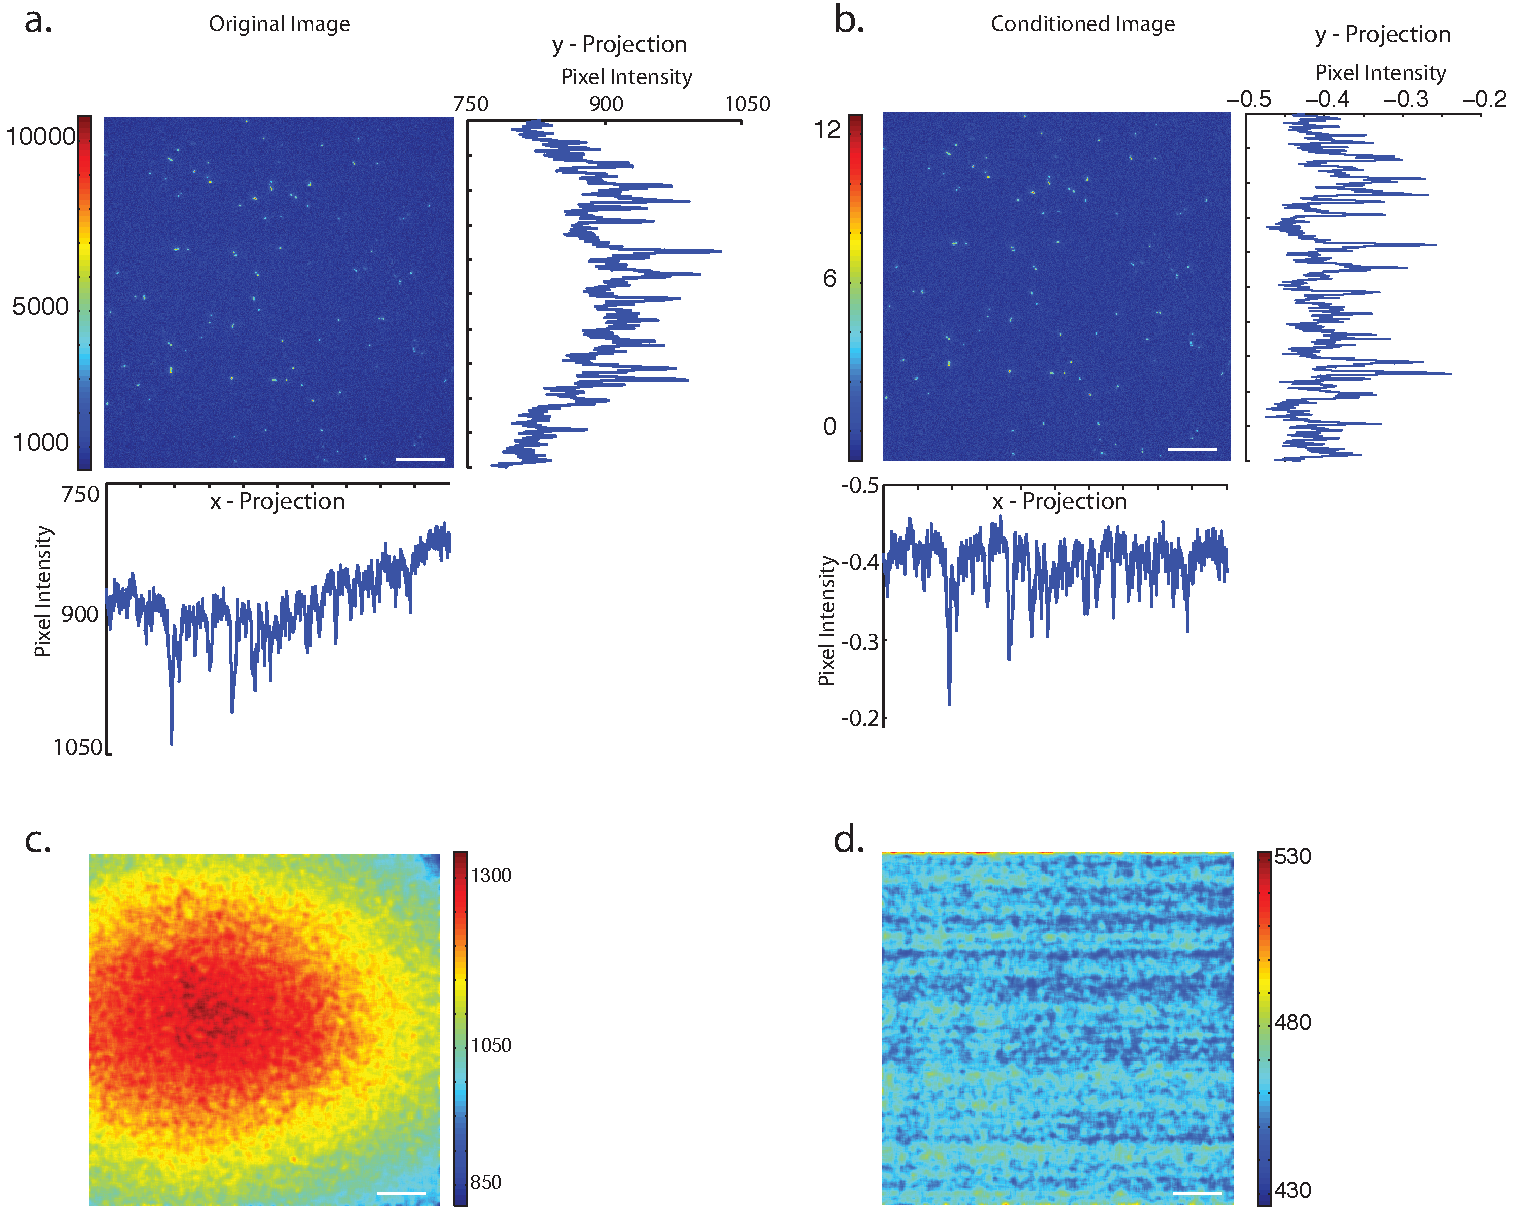
\includegraphics[width=\textwidth]{figures/theoryConditionedImage}
	\caption{The raw image must be conditioned to remove offset and correct scaling. For all images, scalebar is 10 \textmu m.(\textbf{a}) The raw image (1000 px by 1000 px) of DNA origami barcodes (red channel) is shown along with  its projection onto the $x$- and $y$-axes of the image. The raw image has a large offset and the background varies slowly. (\textbf{b}) The conditioned image (red channel) is shown with projections onto the $x$ and $y$ axes. The background of the conditioned image has a mean close to zero, and it does not slowly vary. \textbf{(c)} Image of only the background (red channel). This is the image of slide and buffer without barcodes taken under the same conditions as in \textbf{a}. The glowing spot towards the left reveals uneven illumination. Image has been smoothed by convolution with a Gaussian of width $\sigma=10$ px. This image is used to correct for uneven illumination.   \textbf{(d)} Dark image (red channel) taken without slide or buffer in the absence of illumination is used to correct for DC camera offset. Image has been smoothed by convolution with a Gaussian of width $\sigma=10$ px. \label{fig:conditionedImage}}
\end{center}	
\end{figure}




%We would like to apply the simple model described above to the problem of identifying the barcodes in two-dimensional images. To do so, we perform image processing on the two-dimensional images that transforms them into a one-dimensional form appropriate for the analysis described above. The analysis assumes, as well, that noise in the barcode images is additive, zero-mean and Gaussian. We will show later that the experimentally-observed noise is Gaussian to good approximation. It is clear from inspection, however, that the background of the barcode images does not have zero mean and also has a slowly varying spatial inhomogeneity. To remove this slowly-varying non-zero-mean background, we must account for all of the contributions to the signal recorded by the detector.

The voltage $V(\mathbf{r})$ at a pixel $\mathbf{r}$ in the detector is the sum of a term that is proportional to the number of incident photons, a DC offset $V_0(\mathbf{r})$ that can slowly vary from pixel to pixel, and thermal noise $v_t$ that we assume is Gaussian and zero-mean,
\begin{equation}\label{eq:V_of_r}
V(\mathbf{r})=V_0(\mathbf{r})+c \cdot \text{Photons}(\mathbf{r}) +v_t,
\end{equation}
where $c$ is the conversion constant that relates the number of photons to voltage. 


Recall that, in our system, laser light at one wavelength is incident on the sample and stimulates a fluorophore to emit photons at another wavelength that passes through a narrowband filter to reach the detector. Photons that reach the detector must have been emitted either from fluorophores located  in the barcodes themselves $f$ or from contaminants and impurities in the background media $b$, which consists of a glass slide and buffer.  In both cases, we model the number of photons that are emitted as proportional to the number of incident photons, 

\begin{eqnarray}\label{eq:f_and_b}
f(\mathbf{r})&=&\gamma_{\text{ex}}(\mathbf{r}) q_f(\mathbf{r})\\
b(\mathbf{r})&=&\gamma_{\text{ex}}(\mathbf{r}) q_b.
\end{eqnarray}
Here $\gamma_{\text{ex}}(\mathbf{r})$ is the slowly varying position-dependent intensity of the excitation laser,  $q_f(\mathbf{r})$ describes the position-dependent fluorescent efficiency of the barcodes independent of illumination, and $q_b$ is the background fluorescent efficiency of the media which is assumed to be independent of position and illumination. The term $q_f$ is itself composed of light from fluorophores at positions $\mathbf{r}_i$, each modulated by the point spread function (PSF) $h$ of the optical system

\begin{equation} \label{eq:withPSF}
q_f(\mathbf{r})=\sum_j a_j \delta(\mathbf{r}-\mathbf{r}_j) * h(\mathbf{r}).
\end{equation}
Here $a_j$ is a factor that accounts for intensity variations due to inconsistant fluorescent labeling  during barcode assembly and the star denotes the convolution operation.

The contributions of the terms in Eq.~\ref{eq:V_of_r} can be evaluated by acquiring auxiliary images. The offset and thermal detector noise are present in a dark image taken when the laser is off, for example, and the background media noise and spatially varying illumination become visible in an image taken with the laser on and with media present but with no barcode samples. The final image, of course, has all of these plus DNA barcodes in the media. The voltages recorded in these cases are
\begin{eqnarray}
V_{\text{dark}}(\mathbf{r})&=&V_0(\mathbf{r})+v_t\\
V_{\text{back}}(\mathbf{r})&=&V_0(\mathbf{r})+c \cdot  b(\mathbf{r})  +v_t\\
V_{\text{fluor}}(\mathbf{r})&=&V_0(\mathbf{r})+c \cdot \big[ f(\mathbf{r}) + b(\mathbf{r})\big]  +v_t
\end{eqnarray}
corresponding to Figure \ref{fig:conditionedImage}d, c and a, respectively. 

The offset and illumination intensity vary over the length of the image but are constant over the length of a barcode. To characterize the variations while removing rapid noise fluctuations, the dark and background images are smoothed over a length scale large compared to a barcode but small compared to the entire image. These smoothed images are then subtracted and divided, to remove the DC offset and compensate for the spatially varying illumination, respectively, producing a unitless conditioned image (Figure \ref{fig:conditionedImage}b),

\begin{equation}
U(\mathbf{r})= \frac{ V_{\text{fluor}}(\mathbf{r}) - \widetilde{V}_{\text{back}}(\mathbf{r})  }{ \widetilde{V}_{\text{back}}(\mathbf{r}) - \widetilde{V}_{\text{dark}}(\mathbf{r})} ,
\end{equation}
where~$\widetilde{~~}$~denotes smoothing. Substituting Eq.~\ref{eq:f_and_b} gives
\begin{equation}
U(\mathbf{r})= \frac{ c \cdot \big[ f(\mathbf{r})  +b(\mathbf{r}) -\widetilde{b}(\mathbf{r}) \big]+ v_t  }{   c \cdot \widetilde{b}(\mathbf{r}) }
\end{equation}
Note that $\widetilde{V}_0(\mathbf{r}) = V_0(\mathbf{r})$ and $\widetilde{\gamma}_{\text{ex}}(\mathbf{r})  = \gamma_{\text{ex}}(\mathbf{r})$ since both are assumed to be slowly varying. Substituting further, and recalling that the means of the noise terms are zero, gives
\begin{equation}
U(\mathbf{r})= \frac{ c \cdot \gamma_{\text{ex}}(\mathbf{r}) q_f(\mathbf{r})  + v_t  }{ c \gamma_{\text{ex}}(\mathbf{r})  q_b }
\end{equation}
or
\begin{equation}\label{eq:realDeal}
U(\mathbf{r})= \frac{ q_f(\mathbf{r}) }{ q_b}   + \frac{ v_t }{   c \gamma_{\text{ex}}(\mathbf{r}) q_b}.
\end{equation}


The first term is the fundamental fluorophore distribution, the second term is thermal noise scaled by the local intensity of illumination, while the factor $q_b$ is a constant. This conditioned thermal noise term is sufficiently zero-mean, gaussian, and on the length-scale of a barcode is identical independently distributed (IID), as will be verified later.

Now that the spatially varying offset and illumination have been removed, we turn to the problem of barcode identification. Since performing multiple-hypothesis testing on a two-dimensional dataset is computationally intensive, we start with a simple one-dimensional identification problem. 

\subsection{One dimension, single channel}
In the one dimensional problem we assume that there are $K$ possible one-dimensional reference signals in a system with zero-mean additive Gaussian noise $n$, such that for any reference $m_k$, the observed signal $u=m_k+n$. Collecting each signal into a data vector gives
\begin{equation}
\mathbf{u}=\mathbf{m} + \mathbf{n},
\end{equation}
Given a noisy observation $\mathbf{u}$, we seek the most likely corresponding reference or model signal $\mathbf{m}_k$. 

The $a posteriori$, or inverse, probability that the $k$th reference signal $\mathbf{m}_k$ is present when the data vector $\mathbf{u}$ is observed is given by Bayes' theorem,
\begin{equation}\label{eq:Bayes}
p(\mathbf{m}_k|\mathbf{u}) = \frac{p(\mathbf{u}|\mathbf{m}_k)p(\mathbf{m}_k)} {p(\mathbf{u})},
\end{equation}
where $p(\mathbf{u}|\mathbf{m}_k)$ is the forward probability or likelihood of seeing data $\mathbf{u}$ given the presence of model $\mathbf{m}_k$, $p(\mathbf{m}_k)$ is the prior probability that model $\mathbf{m}_k$ is present, and $p(\mathbf{u})$ is a normalization constant \citep{bretthorst_probability_2003}. We seek to compute the inverse probability for each possible reference $\mathbf{m}_k$, $k=1,2,3 \ldots K$ and select the largest, which is the one most likely to fit the observed data.

While testing a particular observed signal $\mathbf{u}$ against all models, the denominator is constant and independent of $k$. Maximizing $p(\mathbf{m}_k|\mathbf{u})$ is therefore equivalent to finding the model $k$ that maximizes the product  $p(\mathbf{u}|\mathbf{m}_k)p(\mathbf{m}_k)$.
In the present case where all barcodes are equally probable,
$p(\mathbf{m}_k)=1/K$ 
and the search simplifies to finding the maximum likelihood 
\begin{equation}
L_k = p(\mathbf{u}|\mathbf{m}_k).
\end{equation}
This is termed the maximum likelihood solution.


The probability $p(\mathbf{u}|\mathbf{m}_k)$ of observing $\mathbf{u}$ given the reference $\mathbf{m}_k$ is simply the probability that the difference $\mathbf{u}-\mathbf{m}_k$ between the signal and the reference is generated by noise. This is given by the multivariate probability density function for the random Gaussian variable $(\mathbf{u}-\mathbf{m}_k)$, 
\begin{equation}\label{eq:Main}
L_k = p(\mathbf{u}|\mathbf{m}_k) = \frac{1}{  \sqrt{ (2\pi)^N \det || \mathbf{R}_n||} } \exp\left[ -\frac{1}{2}  (\mathbf{u}-\mathbf{m}_k)^T \mathbf{R}_n^{-1} (\mathbf{u}-\mathbf{m}_k) \right]
\end{equation}
where $N$ is the length of vector $\mathbf{u}$, $\mathbf{R}_n$ is the noise covariance matrix, $\det||{\cdot}||$ is the matrix determinant, and $T$ denotes the transpose operation  \citep{helstrom_statistical_1968, wainstein_extraction_1962}.

For the case of identical independently distributed (IID) Gaussian noise, 
\begin{equation}
\mathbf{R}_n=\sigma^2 \mathbf{I}
\end{equation}
where $\mathbf{I}$ is the identity matrix and $\sigma^2$ is the variance of the noise. The probability thus reduces further to
\begin{equation}\label{eq:iidEnergy}
L_k = p(\mathbf{u}|\mathbf{m}_k) = \frac{1}{  \sigma^N \sqrt{ (2\pi)^N}   } \exp\left[ -\frac{(\mathbf{u}-\mathbf{m}_k)^T(\mathbf{u}-\mathbf{m}_k)} {2 N \sigma^2 } \right].
\end{equation}

The exponent is simply the energy contained in the sequence $\mathbf{u}-\mathbf{m}_k$ divided by the
energy of a sequence of noise of length $N$ and variance $\sigma^2$. We recognize parallels to the Maxwell-Boltzmann distribution of statistical mechanics \citep{reif_fundamentals_1965} whereby high-energy sequences (in this case ones where the model is a poor match to the observed signal) are unlikely to be generated by random noise.  

As mentioned, we find the $\mathbf{m}_k$, or rather just the index $k$, that produces the maximum likelihood in equation \ref{eq:iidEnergy}, that is,
\begin{equation}
\max_k   \left\{ p(\mathbf{u}|\mathbf{m}_k) \right\} =  \max_k  \left\{ \frac{1}{   \sigma^N\sqrt{ (2\pi)^N}  } \exp\left[ -\frac{(\mathbf{u}-\mathbf{m}_k)^T(\mathbf{u}-\mathbf{m}_k)} {2 N \sigma^2 } \right] \right\}. 
\end{equation}
This equation leads directly to implementation with a classic matched filter ADD REFS [WAIN62], [HELS68]. 

This equation has another interpretation, as well. Since $\sigma$ and $N$ are independent of $k$ and since the exponential is a monotonically increasing function of its argument, maximizing the likelihood across $k$ is equivalent to minimizing the energy of the difference between the observation and the reference across $k$ 

\begin{equation}
\max_k   \left\{ p(\mathbf{m}_k|\mathbf{u}) \right\} = \min_k  \left\{ (\mathbf{u}-\mathbf{m}_k)^T(\mathbf{u}-\mathbf{m}_k) \right\}. 
\end{equation}
Note that the Bayesian hypothesis test is equivalent in this case to finding the $k$ that minimizes the mean squared error between observation and reference. This is clear by rewriting this expression explicitly in terms of a sum,
\begin{equation}
\max_k   \left\{ p(\mathbf{m}_k|\mathbf{u}) \right\} =  \min_k  \left\{ \sum_{i=1}^N  (u_i-m_{k,i})^2   \right\}. 
\end{equation}
Thus, for the one-dimensional barcode case, the Bayesian hypothesis test is equivalent to classic matched filter and least-mean-squared-error (LMSE) detection strategies.

\subsection{One dimension, multiple channels}\label{sec:simpleModel}
We now consider a system where each reference $\mathbf{m}_k$ consists of three one-dimensional vectors $\mathbf{m}_{k1}$, $\mathbf{m}_{k2}$ and $\mathbf{m}_{k3}$ each of length $N$. Each will correspond to the portion of the reference contained in a different channel, so there are still $K$ references. Analogously, the signal $\mathbf{u}$ also consists of three one-dimensional observations $\mathbf{u}_1$, $\mathbf{u}_2$ and $\mathbf{u}_3$, each in its own channel, and each channel has zero-mean additive IID Gaussian noise with variances $\sigma_1^2$, $\sigma_2^2$ and $\sigma_3^2$, respectively. As we will see later, these channels can be thought of as the red, green and blue channels in a one-dimensional composite color image. 

Because the three channels are independent, the likelihood that signal $\mathbf{u}$ is observed when $\mathbf{m}_k$ is present simply factors into the product of the individual likelihoods, namely, it is the likelihood that $\mathbf{u}_1$ is observed when $\mathbf{m}_{k1}$ is present times the likelihood that $\mathbf{u}_2$ is observed when $\mathbf{m}_{k2}$ is present times the likelihood that $\mathbf{u}_3$ is observed when $\mathbf{m}_{k3}$ is present \citep{bretthorst_probability_2003},
\begin{equation}
p(\mathbf{u}|\mathbf{m}_k) = p(\mathbf{u}_1|\mathbf{m}_{k1})p(\mathbf{u}_2|\mathbf{m}_{k2})p(\mathbf{u}_3|\mathbf{m}_{k3}).
\end{equation}

Substituting Eq.~\ref{eq:iidEnergy} gives
\begin{multline}
L_k=p(\mathbf{u}|\mathbf{m}_k) =\frac{1}{ (\sigma_1\sigma_2\sigma_3)^N  (2\pi)^{3N/2}  }  \exp\Bigg[ -\frac{(\mathbf{u}-\mathbf{m}_{k1})^T(\mathbf{u}-\mathbf{m}_{k1})} {2 N \sigma_1^2 }   - \\ \frac{(\mathbf{u}-\mathbf{m}_{k2})^T(\mathbf{u}-\mathbf{m}_{k2})} {2 N \sigma_2^2 } -\frac{(\mathbf{u}-\mathbf{m}_{k3})^T(\mathbf{u}-\mathbf{m}_{k3})} {2 N \sigma_3^2 }    \Bigg].
\end{multline}

As before, we can factor out and ignore terms that have no $k$ dependence. Thus the maximum likelihood model $k$ correspond to finding $k$ that minimizes the quantity on the right below:
\begin{multline}\label{eq:mle}
\max_k   \big\{ p(\mathbf{m}_k|\mathbf{u}) \big\} =  \min_k  \Bigg\{  \frac{(\mathbf{u}_1-\mathbf{m}_{k1})^T(u_1-\mathbf{m}_{k1})}{\sigma_1^2} +\\  
\frac{(\mathbf{u}_2-\mathbf{m}_{k2})^T(\mathbf{u}_2-\mathbf{m}_{k2})}{\sigma_2^2} + \frac{(\mathbf{u}_3-\mathbf{m}_{k3})^T(\mathbf{u}_3-\mathbf{m}_{k3})}{\sigma_3^2} \Bigg\}. 
\end{multline}
This is the best solution to finding the identity of the barcode.

\section{Implementation}
To identify and decode our barcodes, we start with three conditioned images, $U_1(\mathbf{r}), U_2(\mathbf{r}), U_3(\mathbf{r})$, one each for channel Red, Green, and Blue, respectively.  Before we can begin to employ the solution in Eq.~\ref{eq:mle}, we must locate the barcodes within our image, normalize the intensities of the barcodes across the three channels, and project the barcodes down to a single dimension. Each of these steps requires multiple sequential image manipulations which are described in detail in the next three sections. At the conclusion of the first, Section \ref{sec:projectDown}, we will  have one-dimensional 3-channel projections of our barcodes. Section \ref{sec:generateReferences} describes how the reference signals are generated. Finally, in Section \ref{sec:compareSignal2Ref} the barcodes are decoded by comparing the observed signals with the generated references  using Eq.~\ref{eq:mle}.

\subsection{Locating the Barcodes} \label{sec:locatingBarcodes}
Before we can decode the barcodes, we first must locate them in our image. We locate the barcodes by thresholding away background noise, and studying the morphology of the remaining bright image features. Finally, we apply selection criteria to select out only image features that match the shape of a barcode (see Figure \ref{fig:blobs}). 

\begin{FPfigure}
	\includegraphics[width=\textwidth]{figures/theoryBlobRelated}
	\caption{Image processing is used to locate barcodes and to normalize the intensity across the three channels. Scale bar is 100 \textmu m.
	\textbf{(a)} The conditioned image of the barcodes is shown. The three color channels have been merged into a single channel. Color indicates intensity. 
	\textbf{(b)} Each channel of the conditioned image in \textbf{a} has been  smoothed by convolution with a Gaussian of width less than that of the average peak width. This decreases noise for thresholding. The three smoothed color channels are shown here merged together, where color indicates intensity. 
	\textbf{(c)} Each channel of the smoothed conditioned image in \textbf{b} is thresholded according to a channel-specific user-specified threshold. The three binary images, one each for channel Red, Green and Blue,  are shown in a composite image.  By inspecting the thresholded regions in each color channel, the software can measure the mean peak height for each channel. 
	\textbf{(d)} The union of the three binary images in \textbf{c} is shown as a single binary image. Contiguous white patches are called blobs.
	\textbf{(e)} The binary image in \textbf{d} is dilated. This image is used by the software to group nearby blobs in image \textbf{d} together into blob ensembles.  The area and eccentricity of each blob ensemble is inspected, and those that match the criteria of a barcode are flagged as such. Their location and orientation is recorded. 
	\textbf{(f)} The conditioned image normalized by mean peak height in each channel is shown. On average the height of peaks in each channel is unity. Here the the three channels are shown merged as one, where color indicates intensity.  Note how the intensity of fluorescing spots on barcodes is more uniform here than in \textbf{a}.
	Dotted lines indicate the location of blob ensembles from \textbf{d} that match the criteria for barcodes.\label{fig:fig:blobs}}
\end{FPfigure}


 To threshold, we generate a smoothed image $\tilde{U_i}(\mathbf{r})$ for each channel of $U_i$, by  convolution with a gaussian whose width is narrower than that of the point spread function in Eq.~\ref{eq:withPSF}. See  Figure \ref{fig:blobs}b. The user manually selects a threshold $t_i$ for each of the three channels of the smoothed conditioned image to generate a binary mask,
\begin{equation}
	B_i(\mathbf{r}) = \left\{
	\begin{array}{rl}
		 1 & \text{if } \tilde{U_i}(\mathbf{r}) \geq t_i,\\
		 0 & \text{if } \tilde{U_i}(\mathbf{r}) < t_i,
	\end{array} \right. \qquad\text{for } i=1,2,3
\end{equation}
as in Figure \ref{fig:blobs}c. Noise below the threshold is masked out. Recall that unlike the original images, the conditioned images $U_i$  (Figure \ref{fig:blobs}a) have homogeneous zero-mean  background, so a single threshold per channel is sufficient to capture all barcodes. The three channels of binary masks are merged, 
\begin{equation}
B_{\cup}=B_1\cup B_2 \cup B_3, 
\end{equation}
as in Figure \ref{fig:blobs}d. $B_\cup$ consists of many small discontiguous islands, here called blobs, against a masked-away zero background.  Now we seek to locate barcodes by examining the patterns of blobs.

Some barcodes lie entirely within one blob, while others are represented by two or more nearby but distinct blobs. To correctly locate barcodes, we must first  group together adjacent but distinct blobs.  To do so, we dilate the binary mask using standard image processing routines \citep{matlab_version_2010} so that closely spaced blobs run together into single larger blobs, as in Figure \ref{fig:blobs}e. We can label the larger blobs and use them to group together their constituent blobs, so that, if a barcode is made up of two nearby blobs in $B_\cup$, they both will be labeled together as one blob ensemble.

Each blob ensemble can be examined to determine if it represents a barcode. To qualify as a barcode, the area of a blob ensemble and the major and minor axis of the ellipse that fits its second moment must lie in a range consistent with that of a barcode, and the ellipse must be sufficiently elongated or eccentric. Table~\ref{table:morphCriteria} lists the pertinent numerical criteria. 

\begin{table}[htbp] 
\begin{center}
\begin{tabular}{l c}
\multicolumn{2}{c}{\textbf{Morphological Criteria for Barcode}}\\
Parameter & Value \\
\hline
Min Area & 24 px$^2$ \\
Max Area & 134 px$^2$ \\
Min Length of Major Axis  & 14 px$^2$ \\
Min Eccentricity &0.75\\
\hline
\end{tabular}
\end{center}
\caption{Morphological criteria for barcode. Scale: 1 px $\approx$ 71.4 nm.\label{table:morphCriteria}}
\end{table}
The software also records the centroid and the angle of the barcode major axis, which will be used in Section \ref{sec:projectDown} to rotate the barcode and project it to one dimension. 



\subsection{Normalizing Intensity of Each Channel}\label{sec:normalizePeakHeight}
The average barcode intensity can vary across color channels since it depends on such channel-specific characteristics as the fluorophore, illumination wavelength, illumination intensity, and the width of the narrowband filter. These are normalized across channels by dividing the intensity in each channel by the mean peak height in that channel,  $\langle g_i \rangle$, where $i=1,2,3$ denotes the channel number. 

To measure mean peak height, the software first identifies blobs in the binary mask $B_i$ that have an eccentricity and an area consistent with that of a single peak. It then finds the brightest pixel in each blob that matches the criteria described in Table~\ref{table:singlePeak}.

\begin{table}[htbp] 	
\begin{center}
\begin{tabular}{l c}
\multicolumn{2}{c}{\textbf{Criteria for Single Peaks}}\\
Parameter & Value \\
\hline
Max Allowed Eccentricity  & 0.7 \\
Max Area &  Mean of Area of Blobs in $B_i$ \\
\hline
\end{tabular}
\caption{Criteria for determining if a blob represents a single peak. \label{table:singlePeak}}
\end{center}
\end{table}

The resulting conditioned and normalized image (Figure \ref{fig:blobs}f) has barcodes with pixel intensities such that the brightest pixel in an average barcode in any channel will have an intensity of one.  Together with information about the locations of the barcodes (Section \ref{sec:locatingBarcodes}), this normalized and conditioned image can be used to create one dimensional barcode intensity profiles (Section \ref{sec:locatingBarcodes}) that can then be decoded using the framework described in Section \ref{sec:simpleModel}.

\subsection{Inspecting the Background}
The decoding framework described in Section \ref{sec:simpleModel} expects zero-mean gaussian background noise. We can inspect the background by masking away the prospective barcodes using the inverse of the binary mask $B_{\cup}$ from Section \ref{sec:locatingBarcodes}. The resulting background has roughly zero mean and Gaussian shape as show in Figure \ref{fig:noisePlots}, and thus is consistent with the assumptions in our model.
\begin{figure}[htbp]
\begin{center}
	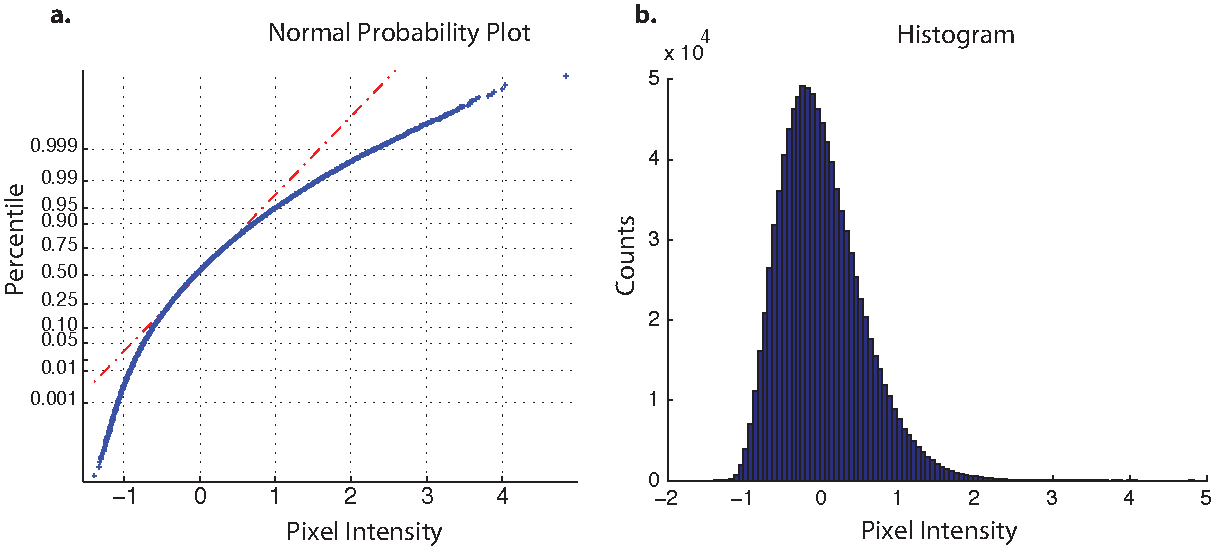
\includegraphics[width=\textwidth]{figures/theoryBackgroundStatistics}
	\caption{The background of the normalized and conditioned image is roughly zero mean and Gaussian.  \textbf{(a)} A normal probability plot compares the cumulative distribution function of the pixel intensities (blue "+" marks) of the background of the red channel of a normalized condition image containing barcodes  with that of a Gaussian (red dashed line.)  \textbf{(b)} Histogram shows number of pixels for given intensity ranges. For both \textbf{a} and \textbf{b} the background pixels were collected from the normalized conditioned image by masking away the location of the barcodes and any other bright fluorescent features.   \label{fig:noisePlots}}
\end{center}	
\end{figure}


   
\subsection{Projecting the Barcode to One Dimension} \label{sec:projectDown}
	To decode a barcode using the one-dimensional matched filter described earlier, we need to first project each three-channel barcode image into three one-dimensional intensity profiles $\mathbf{u}_1, \mathbf{u}_2, \mathbf{u}_3$.  We use the location and orientation of the barcodes found in Section \ref{sec:locatingBarcodes} to rotate the barcode, draw a rectangular bounding box around the barcode and to project it down to a single profile, see Figure \ref{fig:projectDown}.


	\begin{figure}[htbp]
	\begin{center}
		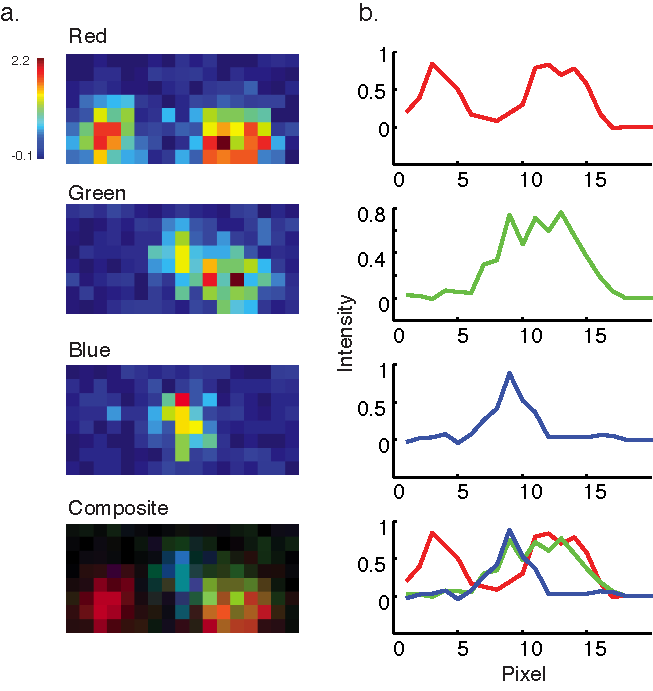
\includegraphics[width=\textwidth]{figures/theoryProjectBarcode}
		\caption{Two-dimensional barcode images are projected down to a single dimension. 1 px $\approx$ 71.4nm. \textbf{(a)}  A single barcode is shown. From top to bottom, the Red, Green,  Blue and a composite image are shown.These images have already been conditioned and normalized. \textbf{(b)} The one-dimensional projections of the images in \textbf{a} are shown. \label{fig:projectDown}}
	\end{center}	
	\end{figure}



  For a given barcode, we first rotate each channel of the  conditioned image $U_i(x,y)$ around the barcode's centroid until the major axis of the barcode lies along the $x$ axis. We call this rotated image  $U_{\theta,i}(x,y)$. The one-dimensional projection of a barcode in the $i$th color channel is then, 
\begin{equation}\label{eq:projectDown}
	   \mathbf{u}_i=u_i(x)=\frac{1}{(y_{\text{max}}-y_{\text{min}})\kappa\langle g_i \rangle}  \int_{y_{\text{min}}}^{y_{\text{max}}} { {U_{\theta,i}(x,y) \mathrm{d}y} },
\end{equation}
where $\langle g \rangle_i$ is the average peak height for this channel described in Section \ref{sec:normalizePeakHeight}, the rectangular region extends from $y_{\text{min}}$ to $y_{\text{max}}$ in the vertical direction, and $\kappa$ is a correction factor, the same for all channels, so that the average peak height remains unity even after the projection. $\kappa$ is the integral of the point spread function $h$ in the vertical direction
\begin{equation}
	\kappa=\int_{-r_0}^{r_0} h(y) \, \mathrm{d}y
\end{equation}
over a preset radius $r_0$ that captures the majority of the energy within $h$. Our analysis models the point spread function $h$ as a gaussian with width $\sigma_{\text{psf}}$,
\begin{equation}\label{eq:psf}
h(r)=\exp \left(  -\frac{r^2}{2\sigma_{\text{psf}}^2} \right),
\end{equation}
so $\kappa$ is
\begin{equation}
\kappa = \frac{\sqrt{2\pi}} {2r_0} \text{erf} \left(\frac{r_0}{2\sqrt{2}\sigma_{\text{psf}}} \right)
\end{equation}
where $\text{erf}$ is the error function \citep{reif_fundamentals_1965}
\begin{equation}
\text{erf}(z) = \frac{2}{\sqrt{\pi}} \int_0^z \exp (-t^2) \, \mathrm{d}t.
\end{equation}

Eq. \ref{eq:projectDown} provides us with three one-dimensional projections of the barcode intensity with average peak heights of unity and with identical independently distributed (IID) zero-mean gaussian noise. These projections are now ready to be compared to a reference to decode the barcode.

\subsection{Generating References}\label{sec:generateReferences}
The last ingredient needed for detection and identification is a bank of reference barcodes to compare against the observed signal. Each reference barcode consists of three one-dimensional traces containing  gaussian peaks of height unity (Eq.~\ref{eq:psf}) superposed at the predicted locations of the fluorescent spots, as shown for example in Fig.~FIGURE WITH PICTURE OF THREE TRACES. 


Although there are only $6^3=216$ species of barcodes, the reference bank must be larger to accomodate the many differences in geometry, or microconfigurations, that the barcode can adopt, including:
\begin{enumerate}
\item left/right reflections, that is, the small gap can lie to the left or to the right,
\item left/right mis-centering within the rectangular window,
\item variation in the fluorophore spacings arising from the barcode manufacturing process, and
\item bends in the DNA strand resulting in a mild U rather than a linear shape.
\end{enumerate}
These differences are accounted for by varying each barcode reference waveform in half-pixel increments, so that the observed profile $\mathbf{u}$ is compared to a bank of references encompassing each possible geometric microconfiguration. Excluding left/right mis-centerings, there are 48 variations that each of the 216 barcode species might adopt, for a total of 10,368 three-channel waveforms in the reference bank. Table~\ref{table:reference} lists the parameters that are allowed to vary, together with their ranges. 

\begin{table}[htbp] 	
\begin{center}
\begin{tabular}{l c}
\multicolumn{2}{c}{\textbf{Reference Barcode Properties}}\\
Parameter & Value \\
\hline
Point Spread Function Width  & $\sigma^2=1.59$ px \\
Allowed Lengths for Big Gap &  \{5.5, 6, 6.5, 7, 7.5, 8\} px \\
Allowed Lengths for Little Gap  & \{ 3.5, 4, 4.5, 5 \} px\\
Window Width & 64 px\\
Number of Barcode Species & 216 \\
Number of Microconfigurations & 10,368 \\
\hline
\end{tabular}
\caption{Reference barcode properties. Scale: 1 px $\approx$ 71.4 nm.\label{table:reference}}
\end{center}
\end{table}

Left/right translations are handled by the circular convolution operation described in the following Section, DELETE THE REFERENCE? \ref{sec:convoloution}  and the bank of references is then used in the multiple hypothesis test of Section INSERT REFERENCE HERE to determine the most likely barcode corresponding to a given observed signal.


\subsection{Decoding the Barcode}
The image processing steps described to this point have prepared the signals for decoding, which is the main task of the software and which we now describe.  We test a given observed signal $\mathbf{u}$ composed of three one-dimensional traces as in Eq. 
\ref{eq:projectDown}, against all 10,368 references, using Eq.~\ref{eq:mle} to identify the most likely one. Expanding this equation for the $i$th channel gives

\begin{equation}
\max_k   \big\{  p(\mathbf{m}_k|\mathbf{u}) \big\} =  \max_k  \Bigg\{ \sum_{i=1}^3  \frac{  2 \mathbf{u}_i ^T \mathbf{m}_{ki} - \lVert \mathbf{u}_i \rVert^2  - \lVert \mathbf{m}_{ki} \rVert^2   }{\sigma_i^2}  \Bigg\}, 
\end{equation}
where $\mathbf{m}_{ki}$  is the $k$th reference and $\sigma_i$ the noise, both in the $i$th channel. Note that $\lVert \mathbf{u}_i \rVert^2$  is independent of the reference $k$ being used for comparison and can be omitted from the maximization, so that
\begin{equation}
\max_k   \big\{  p(\mathbf{m}_k|\mathbf{u}) \big\} =  \max_k  \Bigg\{ \sum_{i=1}^3  \frac{  2 \mathbf{u}_i ^T \mathbf{m}_{ki}  - \lVert \mathbf{m}_{ki} \rVert^2   }{\sigma_i^2}  \Bigg\}. 
\end{equation}
As noted earlier, this equation describes a classic multi-hypothesis matched filter ADD HELSTROM REFERENCE.

Our work would be complete at this point, were it not for possible left/right mis-centering of the barcodes within the rectangular window, as mentioned in  Section \ref{sec:generateReferences}. Instead of adding  additional references to account for all possible translations of all 10,368 references so far, we note that $\mathbf{u}_i ^T \mathbf{m}_{ki}$ is a convolution and translations in the barcode correspond to $x$ offsets or $lags$ between the reference and signal. Symbolically we write this as 
\begin{equation}
\max_k   \big\{  p(\mathbf{m}_k|\mathbf{u}) \big\} =  \max_k  \Bigg\{ \sum_{i=1}^3 \frac{  \max_{x} 2 (\mathbf{u}_i * \mathbf{m}_{ki}) - \lVert \mathbf{m}_{ki} \rVert^2   }{\sigma_i^2}  
\Bigg\},
\end{equation}
where $*$ denotes convolution, and choose the lag that produces the largest result.  It is computationally efficient to calculate such a convolution, for all values of lag, by employing the Fast Fourier Transform. The observed one-dimensional profile $\mathbf{u}_i$ is zero-padded to equal the length of the reference. It and the reference $\mathbf{m}_k$ are transformed, their spectra multiplied, and the product inverse transformed to find the result NEED REFERENCE HERE [Oppe75]. Moreover, the Fourier transform of each reference $m_k$ can be calculated ahead of time just once, and stored together with $\lVert \mathbf{m}_{ki} \rVert^2 / \sigma_i^2$, for use in testing all barcodes in the image.  


\section{Sources of Error}

\subsection{Barcode Defects}
DNA origami barcodes are a nascent technology that will surely see rapid improvements in manufacturing robustness and quality. Using the initial protocol for barcode manufacture as described in Chapter \ref{chapter:DNAbarcode}, we see predominantly two types of barcode defects. First, we see barcodes that have the wrong number of fluorescent spots, either only two spots, or four spots or more. This is likely the result of a barcode that folded improperly or of two barcodes that became conjoined together. The software usually rejects these barcodes based on their morphology, but occasionally the defect conspires to have roughly the same shape as a regular barcode and thus the algorithm is fooled into decoding them. Secondly, we see a more subtle defect. Sometimes two spots in the same color channel on one barcode will vary dramatically in intensity, by as much as 4-fold. Careful inspection by eye will reveal a very bright and very dim spot. This is likely caused by poor labeling of the fluorescent spot. Each spot should have six fluorophores, but we suspect that often the number of fluorophores is less. We evaluate the effectiveness of our software both including and excluding these two classes of defects.    


\subsection{Imaging Conditions}
Our model does not take into account stage drift that may cause slight misalignment between frames. 
Temperature changes in the room, Nor sparodic changes in laser intensity on a \textasciitilde1 minute time scale. Changes slower than \textasciitilde1 are corrected for by taking new regular background and blank images.
 
\section{Software}
The software consists of Matlab scripts tested using MATLAB Version 7.11.0.584 (R2010b) \citep{matlab_version_2010}. The software depends on functions from the following toolboxes: Image Processing Toolbox Version 7.1, Fuzzy Logic Toolbox Version 2.2.12 and Signal Processing Toolbox Version 6.14. The software is released under the GNU General Public License and is available to download from \url{http://github.com/aleifer/DNAbarcode}.

\section{Results}

\begin{figure}[htbp]
\begin{center}
	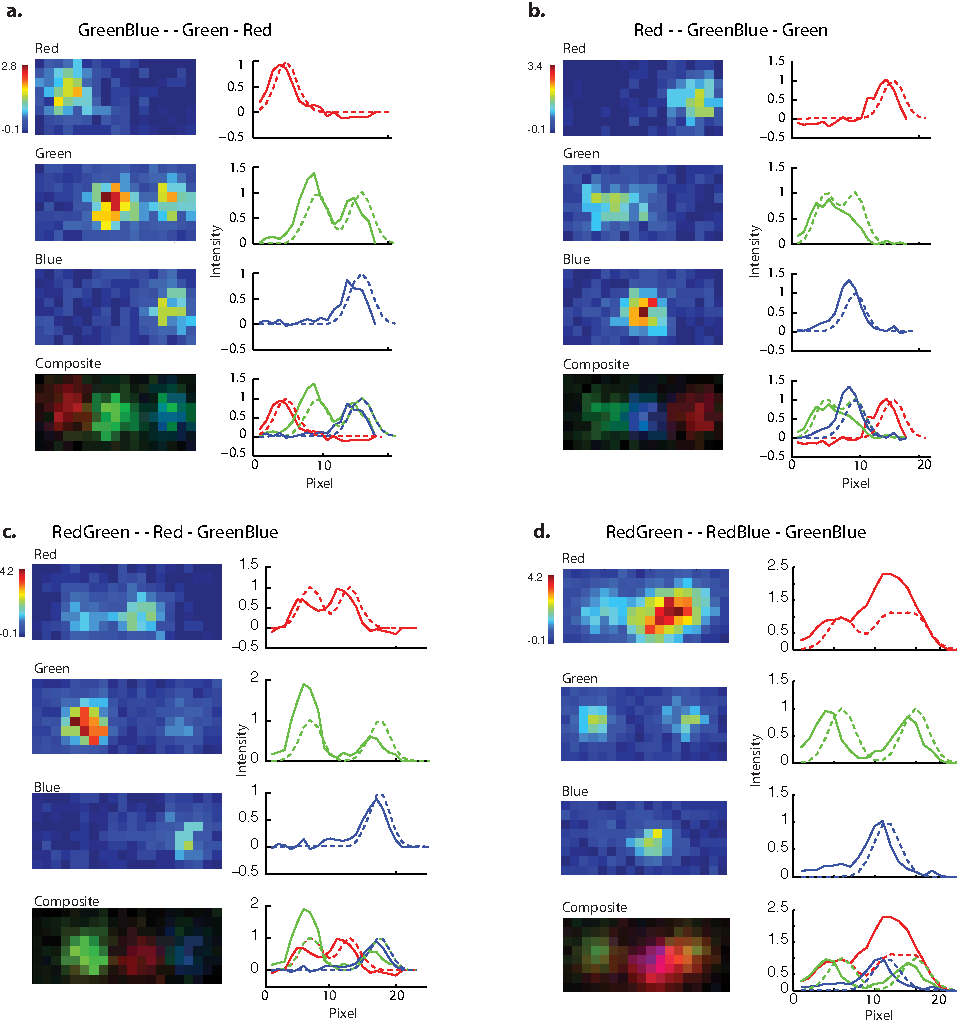
\includegraphics[width=\textwidth]{figures/theoryFittedBarcodes}
	\caption{The software decodes barcodes (solid line) by correctly identifying the most likely reference (dashed line). Four representative barcodes are shown. In each case the software correctly decodes them. The barcodes in \textbf{(a)} and  \textbf{(b)} are well formed and have consistent fluorescent labeling ( peak heights fall between 0.75 and 1.5). The barcodes in \textbf{(c)} and  \textbf{(d)} have peaks that vary widely, even within a channel. This is likely caused by poor labeling during the manufacturing process. \label{fig:fittedBarcodes}}
\end{center}	
\end{figure}




\section{Discussion}


\section{Manuscript Information}
\subsection{Submitted for Publication As}
A version of this chapter has been submitted for publication in the journal \textit{Bioinformatics}.
% in \citep{leifer_optogenetic_2011}:
%\bibentry{leifer_optogenetic_2011}

\subsection{The Author's Contribution}
Andrew M.~Leifer wrote all of the software, generated all figures, developed portions of the mathematical framework, and wrote the majority of the manuscript. Mark C.~Leifer developed portions of the mathematical framework and wrote portions of the manuscript. Chenxiang Lin created the DNA origami barcodes and conducted all microscopy work. 
 